%\part{La Transformada de Laplace}

%{Tabla de contenidos}
% \tableofcontents
%


\section{La Transformada de Laplace}

\subsection{Definici\'on}


 Sea $f(x)$ una funci\'on definida en $0\leq x < \infty$ y sea $s$ una variable arbitraria.  La \emph{Transformada de Laplace} de $f(x),$ denotada ya sea por $\lap{f(x)}$ o por $F(s)$ está dada por
 \[
  \label{bron:21.1}
  \lap{f(x)}=F(s)=\int_{0}^{\infty}e^{-sx}f(x)dx,
 \]
siempre y cuando dicha integral converja.


{}
La convergencia ocurre cuando el límite
\begin{align}
\label{bron:21.2}
\lim_{R\to \infty}
\int_{0}^{R} e^{-sx}f(x)dx
\end{align}
existe.

{}
\begin{observacion}
 \begin{enumerate}
  \item Si el límite anterior no existe, la integral impropia diverge y $f(x)$ no tiene transformada de Laplace.
  \item Cuando evaluamos la integral en \eqref{bron:21.2}, la variable $s$ deberá tratarse como una constante debido a que la integración es respecto de $x.$
 \end{enumerate}

\end{observacion}




 En esta secci\'on usaremos la convención de que una función se denota por minúsculas, mientras que su transformada se denotará por la correspondiente mayúscula:
 $$\lap{f(x)}=F(s),\lap{g(x)}=G(s).$$

 De manera similar, $a,c_{1},c_{2}$ serán constantes arbitrarias.


\subsection{Ejemplos}


 \begin{problema}
  \label{bron:exmp:21.4}
  Encuentre la Transformada de Laplace de
  $f(x)=1.$
 \end{problema}




 \begin{problema}
  \label{bron:exmp:21.9}
  Encuentre la Transformada de Laplace
  $$f(x)=\begin{cases}
     -1 & x\leq 4\\
     1 & x>4
    \end{cases}
$$
 \end{problema}




 \begin{figure}
 \centering
 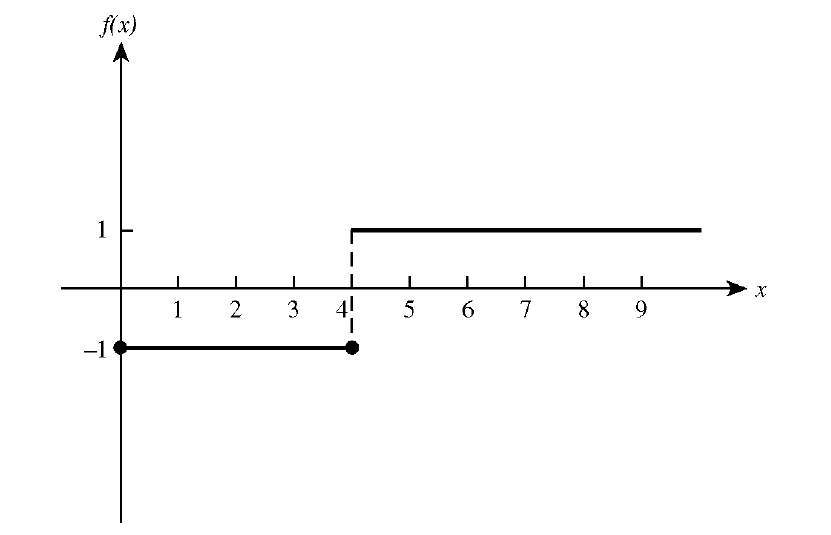
\includegraphics[height=5cm,keepaspectratio=true]{./edo/img0401.png}
 % img0401.png: 0x0 pixel, 300dpi, 0.00x0.00 cm, bb=
 \label{fig:0401}
\end{figure}


{Algunas fórmulas básicas}
\begin{align}
 \label{lap:11}
 \lap{t^{n}} &= \dfrac{n!}{s^{n+1}}, \; \texttt{n natural} \\
 \label{lap:13}
 \lap{\sin(kt)}&=\dfrac{k}{s^2+k^2} \\
 \label{lap:14}
 \lap{\cos(kt)}&=\dfrac{s}{s^2+k^2} \\
 \label{lap:15}
 \lap{e^{at}}&=\frac{1}{s-a}
\end{align}



{Linealidad}
\begin{align}
  \label{bron:21.3}
  \tag{PTL1}
  \lap{c_{1}f(x)+c_{2}g(x)}=c_{1}F(s)+c_{2}G(s)
\end{align}



 \begin{problema}
 \label{bron:exmp:21.10}
 Encuentre la Transformada de Laplace de $f(x)=3+2x^{2}.$
 \end{problema}



 \begin{problema}
  \label{bron:exmp:21.11}
  Encuentre la Transformada de Laplace de
  $$f(x)=5\sin(3x)-17e^{-2x}$$
 \end{problema}




 \begin{problema}
  \label{bron:exmp:21.12}
  Encuentre la Transformada de Laplace de
  $$f(x)=2\sin(x)+3\cos(2x).$$
 \end{problema}




 \begin{problema}
  \label{bron:exmp:21.13}
  Encuentre la Transformada de Laplace de
  $$f(x)=2x^{2}-3x+4.$$
 \end{problema}



\subsection{Propiedades}

\subsection{Propiedades de la Transformada de Laplace}
\begin{align*}
  \label{bron:21.4}
  \tag{PTL2}
  \lap{e^{ax}f(x)}&=F(s-a)\\
  \label{bron:21.5}
  \tag{PTL3}
  \lap{x^{n}f(x)}&=(-1)^{n}\dfrac{d^{n}}{ds^{n}}\left( F(s) \right)
\end{align*}


%
%
% Si $\lim_{x\to 0^{+}}\dfrac{f(x)}{x}$ existe, entonces
% \[
%    \label{bron:21.6}
%    \tag{PTL4}
%  \lap{\frac{1}{x}f(x)}=\int_{s}^{\infty}F(t)dt.
% \]
%
%
%
%
% De manera reciproca,
% \[
%  \label{bron:21.7}
%  \tag{PTL5}
%  \lap{\int_{0}^{x}f(t)dt}=\dfrac{1}{s}F(s).
% \]
%
%

%
% Si $f(x)$ es peri\'odica con periodo $\om,$ es decir $f(x+\om)=f(x), \, \om\neq 0,$ entonces
% \[
%  \label{bron:21.8}
%  %\tag{PTL6}
%  \lap{f(x)}=
%  \dfrac{\int_{0}^{\om}e^{-sx}f(x)dx}{1-e^{-\om s}}
% \]
%
%


 \begin{problema}
  \label{bron:exmp:21.14}
  Encuentre la Transformada de Laplace de
  $$g(x)=xe^{4x}$$
 \end{problema}


{}
\begin{align*}
\label{tlt:22}
\lap{t^{n}e^{at}} = \dfrac{n!}{\left( s-a \right)^{n+1}}
\end{align*}


 \begin{problema}
  \label{bron:exmp:21.15}
  Encuentre la Transformada de Laplace de
  $$g(x)=e^{-2x}\sin(5x)$$
 \end{problema}




 \begin{problema}
  \label{bron:exmp:21.16}
  Encuentre la Transformada de Laplace de
  $$g(x)=x\cos(\sqrt{7}x).$$
 \end{problema}




 \begin{problema}
  \label{bron:exmp:21.17}
  Encuentre la Transformada de Laplace de
  $$g(x)=e^{-x}x\cos(2x).$$
 \end{problema}





